\section{Container Attack Surface Analysis}
\label{sec:container-attack-surface-analysis}

In containerized environments, security challenges often arise from vulnerabilities within specific components of the architecture. As such, understanding the relationships between the different components, such as container registries, images, runtime, namespaces, cgroups, and various security modules like eBPF, seccomp, and Linux capabilities is crucial for identifying potential attack surfaces. This is where a comprehensive architecture diagram comes into play.

\begin{figure}[t]
  \label{fig:architecture}
  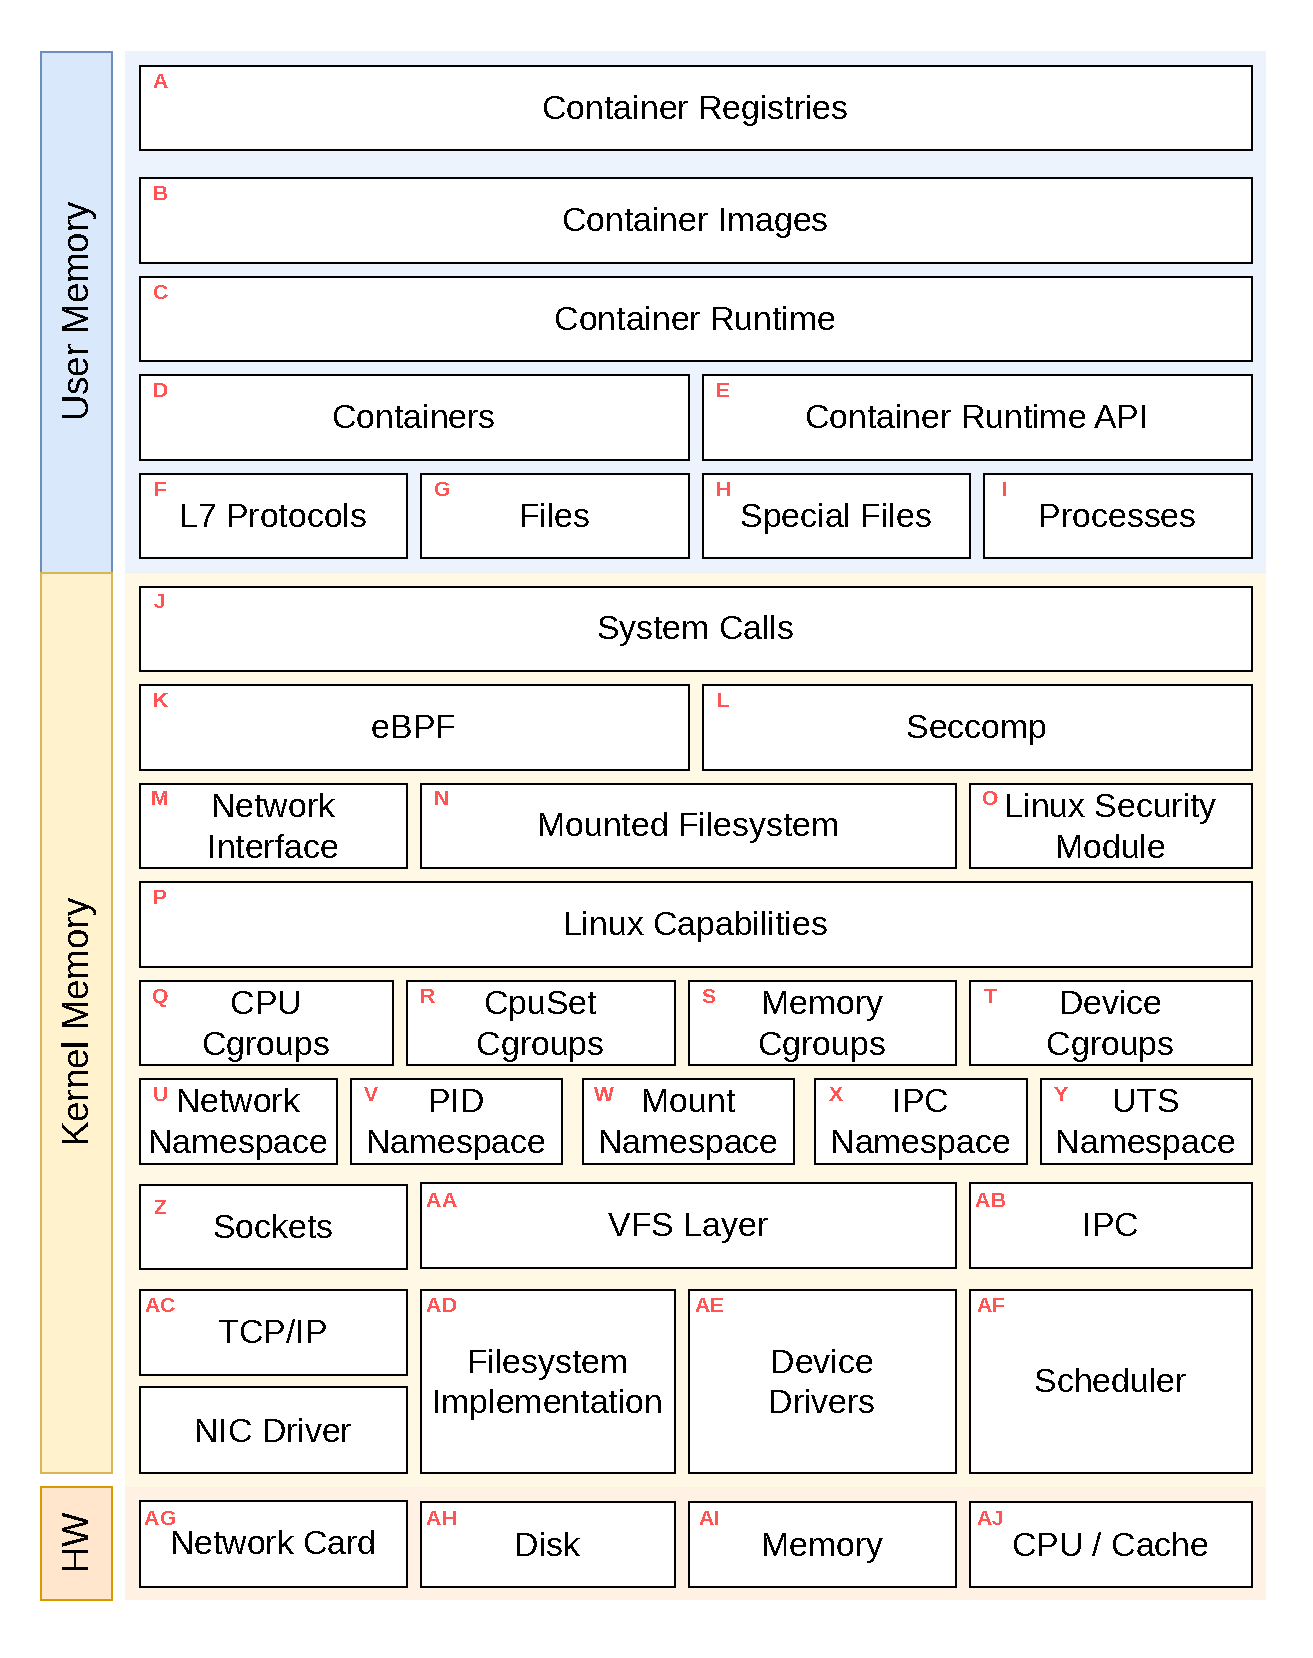
\includegraphics[width=1\linewidth]{figs/exploit-coverage.pdf}
  \caption{An architectural diagram of a container deployment environment depicting the attack surface created by its various components.}
\end{figure}

Figure 2 outlines the key components of a containerized system, highlighting the critical paths and interactions that security tests should focus on. Security testing should aim to cover these components extensively to ensure that vulnerabilities in any of these layers are adequately addressed. However, some components, like network interfaces, system calls, and cgroups, are more frequently targeted in real-world attacks and thus warrant more attention in testing. The diagram will guide our understanding of which components to prioritize during testing, ensuring that our coverage is both thorough and effective.


\section{Evaluation}
\label{sec:evaluation}

To assess the aforementioned security mechanisms, in this section, we evaluate the performance of a series of tricks, such as resource starvation, unauthorized access attempts, and container escapes.

\noindent\textbf{Evaluating DOS Prevention Mechanisms.}

With our first trick, we investigate the resilience of Docker containers against fork bomb attacks, a common form of denial-of-service (DoS) attack, where a process continuously replicates itself, and quickly exhaustes system resources. A fork bomb is designed to overwhelm the process table and exhaust available CPU and memory resources. If a container's resource management policies are inadequate, it would render the system unresponsive in the event of such an attack. Docker is able to leverage various Linux kernel mechanisms, most notably control groups (cgroups), to impose limits on process creation. Therefore, we define the success of this trick if the docker security mechanism that is used can prevent or disallow resource exhaustion. 

In our evaluation of the trick, we applied a value of 10 to the pid\_limit mechanism, which sets a maximum cap on the number of processes that can be created within a container. This configuration was successful in preventing a fork bomb because the container would not be able to create enough processes to exhaust resources.

Cpuset\_cpus, a Docker resource management option, was also tested in this trick to determine its impact on mitigating a fork bomb attack. This setting allows containers to be restricted to specific CPU cores, preventing them from consuming CPU resources system-wide. In our experiment, we set cpuset\_cpus to (1,2), meaning the container was limited to running only on CPU cores 1 and 2.

Even without enforcing a pid\_limit, this configuration effectively contained the fork bomb within the assigned CPU cores, preventing it from overwhelming the system as a whole. The restriction ensured that other cores remained available for critical system processes, reducing the risk of a full system denial-of-service (DoS). This suggests that cpuset\_cpus can serve as an additional mitigation strategy against resource exhaustion attacks by confining CPU-intensive processes to a limited number of cores. However, unlike pid\_limit, which directly limits the number of processes a container can create, cpuset\_cpus does not prevent the fork bomb from executing, it only reduces its impact by isolating it to specific CPU resources.

When no security mechanisms were applied, the fork bomb affected the host OS, the VM guest as well as the container.

\noindent\textbf{Assessing Docker Port Forwarding Restrictions}

For this trick, we will run an HTTP server and bind it to port 23, which is a privileged port. Our objective is to identify which Docker confinement mechanism and versions permit binding port 23 to a process running an HTTP server.

It turns out that Docker made a change starting with version 20.03. They redefined unprivileged ports to start at 0 instead of 1024, which means that the `NET\_BIND\_SERVICE` capability is no longer required to bind to a privlidged port. Thus, we will test one version of docker that is less than 20.03, and one greater than or equal to 20.03.

Starting with the docker version less than 20.03, the results of the tests reveal that binding to a privileged port (port 23) is influenced by several Docker confinement mechanisms. First of all, success was achieved when the `NET\_BIND\_SERVICE` capability was enabled and the user was root. If the NET\_BIND\_SERVICE was activated, but the user was not root, the trick would fail. Other ways the trick could fail is if a custom SECCOMP profile was used to deny the bind system call. This indicates that the ability to bind to privileged ports is primarily dependent on the presence of the `NET\_BIND\_SERVICE` capability and root user privilege. The table below describes these occurences.

\begin{table}
    \centering
    \caption{Effect of Different Security Configurations in Docker versions < 20.03}
    \label{tab:docker-security}
    \small
    \begin{tabular}{|p{6cm}|c|}  % Adjusted second column width
        \hline
        \textbf{Configuration} & \textbf{Result} \\ \hline
        +NET\_BIND\_SERVICE | root & \textcolor{green}{\ding{51}} \\ \hline  % ✅ Success
        -NET\_BIND\_SERVICE | root & \textcolor{red}{\ding{55}} \\ \hline  % ❌ Failure
        +NET\_BIND\_SERVICE | Custom Seccomp (deny bind syscall) + root & \textcolor{red}{\ding{55}} \\ \hline
        -NET\_BIND\_SERVICE | root & \textcolor{red}{\ding{55}} \\ \hline
        +NET\_BIND\_SERVICE | non\_root & \textcolor{red}{\ding{55}} \\ \hline
    \end{tabular}
\end{table}


In Docker versions prior to 20.03, NET\_BIND\_SERVICE had an effect as explained earlier. However, in Docker versions 20.03 and later, NET\_BIND\_SERVICE no longer has any impact. However, root user is still needed to bind the HTTP server to a port, and not nessearily a privlidged port. If the user is a non-root, then the trick will not work. Also, if a custom seccomp profile is used to deny the bind syscall, the trick will not work. All of this is described in the table below.

\begin{table}
    \centering
    \caption{Effect of Different Security Configurations in Docker versions $\geq$ 20.03}
    \label{tab:docker-security}
    \small
    \begin{tabular}{|p{6cm}|c|}  % Adjusted second column width
        \hline
        \textbf{Configuration} & \textbf{Result} \\ \hline
        +NET\_BIND\_SERVICE | root & \textcolor{green}{\ding{51}} \\ \hline  % ✅ Success
        -NET\_BIND\_SERVICE | root & \textcolor{green}{\ding{51}} \\ \hline  % ✅ Success
        +NET\_BIND\_SERVICE | Custom Seccomp (deny bind syscall) + root & \textcolor{red}{\ding{55}} \\ \hline  % ❌ Failure
        +NET\_BIND\_SERVICE | non\_root & \textcolor{red}{\ding{55}} \\ \hline  % ❌ Failure
    \end{tabular}
\end{table}

\noindent\textbf{CVE 2024-21616}


The CVE-2024-21626 vulnerability exists within Docker and runc and allows malicious containers to escape their isolation layer, enabling attackers to take control of the host machine. This poses a significant security risk for enterprises relying on containerization, as once the vulnerability is exploited, attackers could breach security boundaries to access sensitive data and system resources. 

Specifically, the cause of CVE-2024-21626 involves improper setting of the container’s working directory. Under certain conditions, if a container's working directory is set to a special file descriptor path, such as /proc/self/fd/<fd> (where <fd> typically points to the /sys/fs/cgroup directory), it may allow for container escape. The affected versions of runc range from v1.0.0-rc93 to 1.1.11.

To evaluate the practical impact of CVE-2024-21616, we leveraged Houdini to systematically assess the effectiveness of Docker’s confinement mechanisms in preventing container escapes. By integrating CVE-2024-21616 as a Houdini trick, we were able to analyze under what conditions the vulnerability could be exploited and determine the effectiveness of different security configurations in mitigating the risk.

The experiment was structured to evaluate the default security posture of Docker as well as the impact of applying additional confinement measures. The Houdini trick for CVE-2024-21616 was designed using a combination of a configuration file, which defined the container’s security settings, a Dockerfile, which set up the containerized environment, and an exploit script, which attempted to break out of the container and execute arbitrary commands on the host. These files can be seen in section 6.

Our findings revealed that Docker’s default security settings were insufficient to prevent exploitation. The only way to prevent it is to use a runc version greater than 1.1.11. This is because the vulnerability lies inside of runc, the container runtime responsible for managing process execution inside containers. Since the flaw is in the runtime itself, Docker’s built-in security mechanisms, such as namespaces, cgroups, and seccomp, do not inherently prevent exploitation. As a result, even well-configured containers remain vulnerable if they are running on an affected version of runc.


\noindent\textbf{Killing Host Processes}

By default, Docker containers operate in their own isolated process namespace, meaning each container has its own set of processes that it can see and manage. This isolation is one of the fundamental aspects of Docker's security model, preventing containers from interfering with the host system or other containers. Each container runs as if it's a completely separate environment, with its own process tree and PID (process identifier) space.

When you configure a container to run with pid\_mode = host, you effectively remove the process isolation between the container and the host system. In this configuration, the container shares the same process namespace as the host, which means the container can see all processes running on the host, just as a process running natively on the host would. This feature, while useful in some scenarios, also exposes the container to the host's processes, providing the ability to monitor or interact with them.

By leveraging the pid\_mode = host setting, a container can gain access to the host’s process identifiers (PIDs), enabling advanced use cases such as debugging or monitoring processes on the host from within the container. This is a powerful capability, but it also introduces potential risks. With root privileges, we found that a container can use typical Linux commands, like kill or killall, to target and terminate host processes. For instance, if a process x is running on the host with a specific PID of 343, the container can send a termination signal to process x, effectively killing it from within the container. If the pid\_mode does not map to the host, then we are not able to kill a host process from the container.

However, this trick does not work with non-root privileges, as the kill command requires elevated permissions to target processes owned by other users or system processes. Without root access, the container can still see the host's processes but will lack the necessary permissions to terminate them.


\begin{table}
    \centering
    \caption{Effect of Different Security Configurations in Docker versions $\geq$ 20.03}
    \label{tab:docker-security}
    \small
    \begin{tabular}{|p{4cm}|p{1cm}|}  % Adjusted second column width
        \hline
        \textbf{Configuration} & \textbf{Result} \\ \hline
        pid\_mode=host | root & \textcolor{green}{\ding{51}} \\ \hline  % ✅ Success
        pid\_mode=host | non-root & \textcolor{red}{\ding{55}} \\ \hline  % ✅ Success
        pid\_mode=null & \textcolor{red}{\ding{55}} \\ \hline  % ❌ Failure
    \end{tabular}
\end{table}


\begin{table}
  \caption{\todo{table caption}}
  \label{tab:classification}
  \begin{tabular}{lllll}
    \toprule
    \bfseries Trick \normalfont{(See \Cref{fig:architecture})} & Trick Vector \\
    \midrule
    Evaluating DOS Prevention Mechanisms            & V, R, I \\
    Assessing Docker Port Forwarding Restrictions   & M, P \\
    CVE 2024-21616 & C, G, H \\
    Killing Host Processes  & V, I,   \\
    \bottomrule
  \end{tabular}
\end{table}